\documentclass[tikz, border=4pt]{standalone}
\usepackage[T1]{fontenc}
\usepackage{helvet}
\renewcommand{\familydefault}{\sfdefault}
\usetikzlibrary{arrows.meta, fit, positioning}

\definecolor{client}{HTML}{7B4FB3}
\definecolor{gateway}{HTML}{2F6FD0}
\definecolor{server}{HTML}{1E8A7A}
\definecolor{sandbox}{HTML}{3F8F3A}
\definecolor{store}{HTML}{B07A12}

% "fill=." fills the badge with the colour of the surrounding label text.
\newcommand{\step}[1]{%
  \tikz[baseline=(badge.base)]
    \node[circle, fill=., text=white, font=\small\bfseries, inner sep=1.5pt,
          minimum size=4.6mm] (badge) {#1};}
% A step badge followed by its text; further lines align with the first, not under the badge.
\newcommand{\steplabel}[2]{\step{#1}\ \begin{tabular}[t]{@{}l@{}}#2\end{tabular}}
\newcommand{\boxtitle}[1]{\textbf{#1}\\[2pt]}

\tikzset{
  component/.style={
    draw=#1, fill=#1!8, text=black, thick, rounded corners=3pt,
    align=left, font=\small, inner sep=5pt,
    text width=3.8cm, minimum height=2.6cm,
  },
  storage/.style={component=store, text width=4.85cm, minimum height=2cm},
  part/.style={component=sandbox, fill=white, text width=4.65cm, minimum height=1.5cm},
  arrow tip/.tip={Stealth[length=6pt]},
  flow/.style={-arrow tip, very thick, draw=#1},
  flow label/.style={font=\footnotesize, text=#1, align=left, inner sep=3pt},
}

\begin{document}
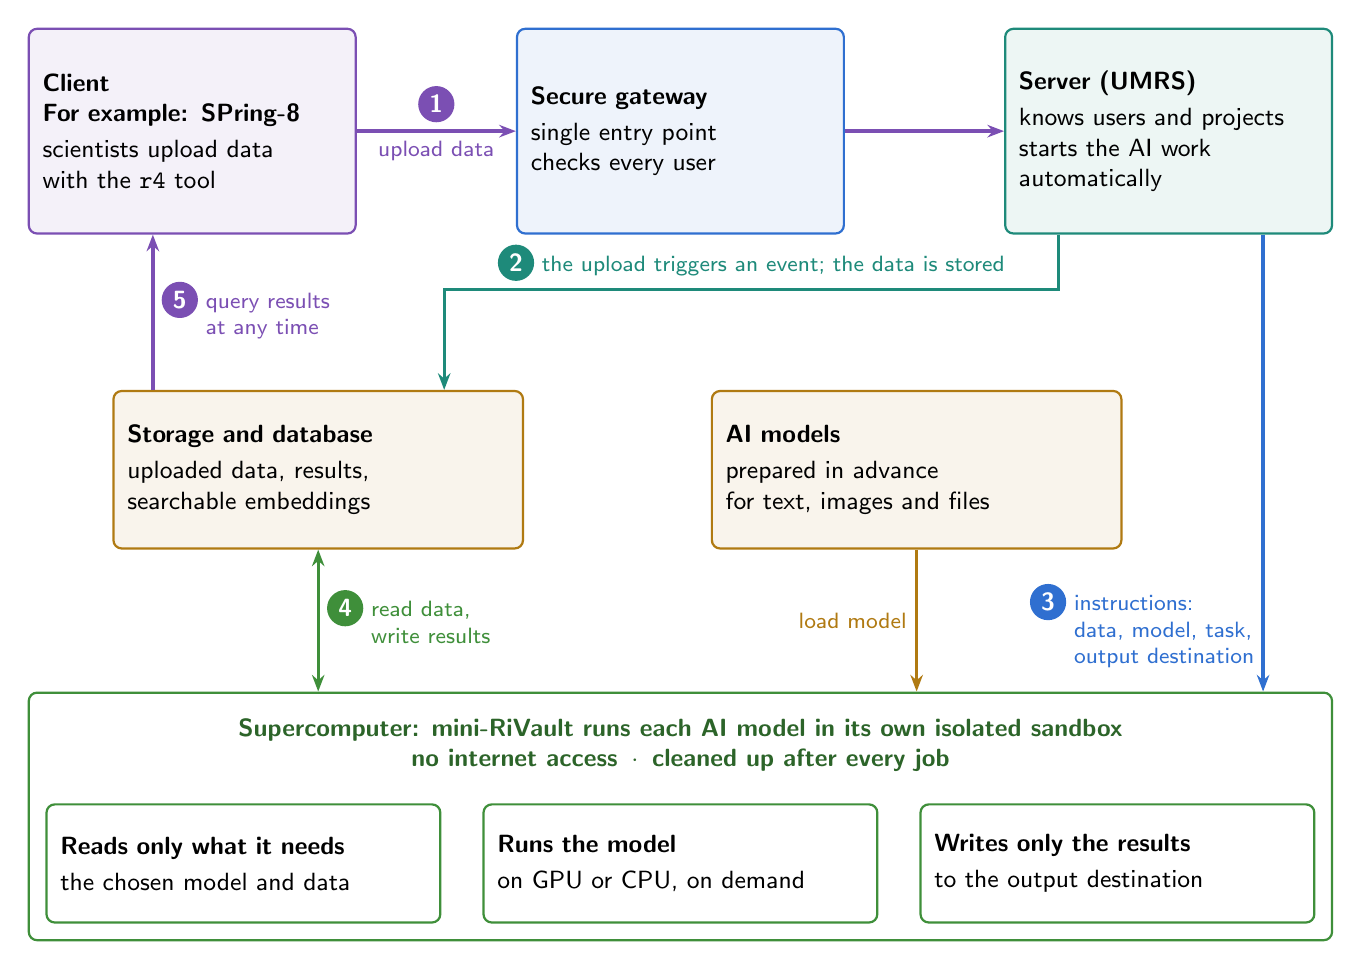
\begin{tikzpicture}
  % Top row: from the scientist to the server.
  \node[component=client] (client) at (0, 0)
    {\boxtitle{Client\\For example: SPring-8}scientists upload data\\with the \texttt{r4} tool};
  \node[component=gateway] (gateway) at (6.2, 0)
    {\boxtitle{Secure gateway}single entry point\\checks every user};
  \node[component=server] (umrs) at (12.4, 0)
    {\boxtitle{Server (UMRS)}knows users and projects\\starts the AI work\\automatically};

  % Middle row: what the AI work needs and produces.
  \node[storage] (storage) at (1.6, -4.3)
    {\boxtitle{Storage and database}uploaded data, results,\\searchable embeddings};
  \node[storage] (models) at (9.2, -4.3)
    {\boxtitle{AI models}prepared in advance\\for text, images and files};

  % Bottom row: where the model runs.
  \node[font=\small\bfseries, text=sandbox!70!black, align=center] (sandbox title) at (6.2, -7.8)
    {Supercomputer: mini-RiVault runs each AI model in its own isolated sandbox\\
     no internet access \,$\cdot$\, cleaned up after every job};
  \node[part] (reads) at (0.65, -9.3)
    {\boxtitle{Reads only what it needs}the chosen model and data};
  \node[part] (runs) at (6.2, -9.3)
    {\boxtitle{Runs the model}on GPU or CPU, on demand};
  \node[part] (writes) at (11.75, -9.3)
    {\boxtitle{Writes only the results}to the output destination};
  \node[draw=sandbox, thick, rounded corners=3pt, inner sep=6pt,
        fit=(sandbox title) (reads) (runs) (writes)] (sandbox) {};

  % Steps of "How to use AIMON" in the readme.
  \draw[flow=client] (client) -- (gateway)
    node[flow label=client, midway, above] {\step{1}}
    node[flow label=client, midway, below] {upload data};
  \draw[flow=client] (gateway) -- (umrs);
  \draw[flow=server] ([xshift=-14mm]umrs.south) -- ++(0, -0.7) -| ([xshift=16mm]storage.north)
    node[flow label=server, pos=0.25, above] {\steplabel{2}{the upload triggers an event; the data is stored}};
  \draw[flow=gateway] ([xshift=12mm]umrs.south) -- ([xshift=12mm]umrs.south |- sandbox.north)
    node[flow label=gateway, pos=0.86, left]
      {\steplabel{3}{instructions:\\data, model, task,\\output destination}};
  \draw[flow=sandbox, arrow tip-arrow tip] (storage.south) -- (storage.south |- sandbox.north)
    node[flow label=sandbox, midway, right] {\steplabel{4}{read data,\\write results}};
  \draw[flow=store] (models.south) -- (models.south |- sandbox.north)
    node[flow label=store, midway, left] {load model};
  \draw[flow=client] ([xshift=-21mm]storage.north) -- ([xshift=-21mm]storage.north |- client.south)
    node[flow label=client, midway, right] {\steplabel{5}{query results\\at any time}};
\end{tikzpicture}
\end{document}
